\section{Complément sur les corps \texorpdfstring{$p$}{p}-adique}
\label{cpadic}

Cette section de l'appendice présente la plupart des preuves qui n'ont pas été traitées en section \ref{padic} ainsi que quelques compléments sur les nombres $p$-adique pour en avoir une meilleur appréhension.


\subsection*{Représentation sous forme d'arbre}
Un façon intuitive de se représenter les nombres $p$-adiques est de les écrire comme les feuilles d'un arbre infini.

<<<<<<< HEAD
On considère l'arbre $\mathcal{T}(\mathbb{Z}_p)$ dont les nœuds sont les suites finies à coefficients dans $\{1,\ldots,p\} $ et tels que deux sommets sont reliés entre eux si et seulement si 
=======
On considère l'arbre $\mathcal{T}(\mathbb{Z}_p)$ dont les nœuds sont les suites finies à coefficients dans $\{1,\ldots,p\} $ et tels que deux sommets $N_1 \to N_2$ sont reliés entre eux si et seulement si $N_1 \subset N_2$ et $|N_2| = |N_1| + 1$. 

On encode alors les $p$-adique comme une suite de sommets reliés entre eux.


\begin{figure}[htpb]
	\centering
	% https://q.uiver.app/#q=WzAsMTUsWzEsMywiMDAiXSxbMCw1LCIwMDAiXSxbMiw1LCIwMDEiXSxbNCwzLCIwMSJdLFszLDUsIjAxMCJdLFs1LDUsIjAxMSJdLFs3LDUsIjEwMCJdLFs5LDUsIjEwMSJdLFsxMCw1LCIxMTAiXSxbMTIsNSwiMTExIl0sWzMsMSwiMCJdLFs4LDMsIjEwIl0sWzExLDMsIjExIl0sWzksMSwiMSJdLFs2LDAsIlxcYnVsbGV0Il0sWzAsMV0sWzAsMl0sWzMsNF0sWzMsNV0sWzEwLDBdLFsxMCwzXSxbMTEsNl0sWzExLDddLFsxMiw4XSxbMTIsOV0sWzEzLDExXSxbMTMsMTJdLFsxNCwxMF0sWzE0LDEzXV0=
\newcommand\lacolora{purple} 
\newcommand\lacouleur{\color{\lacolora}}  
\[\begin{tikzcd}[sep=tiny]
	&&&&&&& \lacouleur{\bullet} \\
	&&&& \lacouleur{0} &&&&&& 1 \\
	\\
	&& 00 &&& \lacouleur{10} &&&& 01 &&& 11 \\
	\\
	&000 && 100 & \lacouleur{010} && 110 && 001 && 101 & 011 && 111\\
	&\vdots && \vdots & \lacouleur{\vdots} && \vdots && \vdots && \vdots & \vdots && \vdots\\
	\hline\\
	\mathbb{Z}_p&      &&& \lacouleur{\ldots011010}&&&&&&&&&
	\arrow[from=4-3, to=6-2]
	\arrow[from=4-3, to=6-4]
	\arrow[from=4-6, to=6-5, \lacolora]
	\arrow[from=4-6, to=6-7]
	\arrow[from=2-5, to=4-3]
	\arrow[from=2-5, to=4-6, \lacolora]
	\arrow[from=4-10, to=6-9]
	\arrow[from=4-10, to=6-11]
	\arrow[from=4-13, to=6-12]
	\arrow[from=4-13, to=6-14]
	\arrow[from=2-11, to=4-10]
	\arrow[from=2-11, to=4-13]
	\arrow[from=1-8, to=2-5, \lacolora]
	\arrow[from=1-8, to=2-11]
\end{tikzcd}\]

 
	\caption{$\mathcal{T}\left( \mathbb{Z}_p \right) $}
	\label{fig:TZp} 
\end{figure}



Cette interprétation en arbre de $\mathbb{Z}_p$ est utile car permet de se figurer certaine propriétés géométriques des $p$-adiques, puisqu'en effet chaque sommet représente exactement une boule 

>>>>>>> afed46df6ee66c8447d25c77be41fc228335ae00

\begin{proof} \hypertarget{qpcorpspreuve}{Proposition \ref{qpcorps}} 
En réalité on dispose même d'un résultat plus précis : $\mathbb{Q}_{p}$ est le corps des fractions de $\mathbb{Z}_p$. Pour prouver ce résultat on utilisera le lemme suivant :
\begin{lemme}
	\label{lemmeinversible} 
	Les inversibles de $\mathbb{Z}_p$ sont exactement les entiers $p$-adique $\overline{\ldots x_n\ldots x_1x_0}$ tels que $x_0$ est non nul.
\end{lemme}
\textit{Preuve du lemme :} 
Un entier $p$-adique $x = \overline{\ldots x_n \ldots x_1 x_0}$ est inversible si et seulement si il est inversible dans $\mathbb{Z}{/p^n\mathbb{Z}}$ pour tout $n \in \mathbb{N}$, c'est-à-dire si et seulement si $ \sum \limits_{i=0}^{n}p^i x_{i}$ est premier avec $p^n$ pour tout $n \in \mathbb{N}$ ce qui est équivalent à $x_0$ premier avec $p$ et donc $x_0 \neq 0$.

Ensuite il suffit de remarquer que tout entier $p$-adique non nul $x = \overline{\ldots x_n \ldots x_1 x_0}$ s'écrit $p^n \tilde{x}$ avec $\tilde{x} \in \mathbb{Z}_p^\times $ et $n$ un entier naturel. On a de plus unicité par \ref{lemmeinversible}. 

En effet, si on pose $n$ le plus petit entier naturel tel que $x_n \neq 0$\footnote{c'est-à-dire la valuation de $x$} et $\tilde{x} := \overline{\ldots x_n }$ on a immédiatement $ x = p^n \tilde{x}$ et $\tilde{x} \in \mathbb{Z}_p^\times $. Il est alors immédiat que $\mathbb{Q}_{p} = \mathbb{Z}_p[\frac{1}{p}]$ est le plus petit corps contenant $\mathbb{Z}_p$

\end{proof}

\begin{proof} \hypertarget{propvalpreuve}{Propriété \ref{propval} }  
	Soient $x,y$ deux entiers naturels de valuation $n := \val\left(x\right)$ et $m := \val\left(y\right)$.
	On peut alors écrire $x = p^n \tilde{x}$ et $y = p^m \tilde{y}$ avec $\tilde{x}, \tilde{y} \in \mathbb{Z}_p^\times $, comme vu \hyperref{qpcorpspreuve}{plus haut}.
	On a alors tout d'abord $xy = (\tilde{x}\tilde{y}) p^{n+m}$ et donc par unicité de la décomposition $\val\left(xy\right) = \val\left(x\right)+\val\left(y\right) $.

Ensuite, on trouve que $x+y \in p^n \mathbb{Z}_p+ p^m \mathbb{Z}_p = p ^{\min\left( m,n \right) }\mathbb{Z}_p $ ce qui signifie que $\val\left(x+y\right)\ge \min\left( \val\left(x\right), \val\left(y\right) \right) $. Puis si $m\neq n$ on peut supposer sans perte de généralité que $m>n$ et $x+y$ s'écrit alors $p^n(p^{m-n} \tilde{x} + \tilde{y})$ et par \ref{lemmeinversible}, $p^{m-n}\tilde{x}+\tilde{y} \in \mathbb{Z}_p^\times$.  
\end{proof}

<<<<<<< HEAD
\begin{proof} \hypertarget{caracsdppreuve}{Théorème \ref{caracsdp} }

=======
\begin{proof} \hypertarget{caractères}{Théorème \ref{caracsdp} }
	
Afin de prouver le théorème \ref{caracsdp} nous allons reformuler ce dernier sous la forme équivalente suivante : 

	\begin{propriete}
		Un polynôme de $\mathbb{Q}_{p} [X] $\emp{unitaire et de terme constant entier}est a uniquement des racines de valuation positive ou nulle dans $\overline{\mathbb{Q}_{p} }$ si et seulement si il est à coefficients dans $\mathbb{Z}_p$. 
	\end{propriete}
Si prouver le sens réciproque de cette équivalence se fait sans difficulté, le sens direct est, lui plus complexe à démontrer. Pour ce faire, nous utiliserons un outil particulièrement utile pour l'étude des polynômes à coefficients $p$-adique : les polygones de Newton.

\textit{Preuve du sens réciproque :} 
	Soit $P = X^n + \sum \limits_{i=0}^{n-1} a_{i} X^i $ un polynôme à coefficients dans $\mathbb{Z}_{p}$. 
	Montrons par l'absurde que toute racine de $P$ est de valuation positive. Soit $\rho \in \overline{\mathbb{Q}_{p} }$ une racine de $P$, supposons $\val\left( \rho\right)<0$. D'après la propriété \ref{propval}, $\val\left(P( \rho)\right) = \min \left( \val\left( \rho^n \right), \val(a_{n-1} \rho^{n-1}),\ldots, \val(a_0) \right)$. Or on a l'inégalité $\val\left( \rho^n\right) = n \val\left( \rho\right)\le \val\left(a_{i} p^{i} \right) = i\val\left( \rho \right) + \val\left(a_{i}\right)$ pour $i=1,\ldots,n$, car $a_i \in \mathbb{Z}_p$. Ainsi $\val\left(P( \rho)\right) = n \val\left( \rho\right) <0$, or $\rho$ est une racine de $P$ et donc $\val\left( P( \rho) \right) = \val\left(0\right) = +\infty$. Ce qui est absurde, donc $\val\left( \rho\right) \ge 0$.

	\textit{Preuve du sens direct :} 

	Pour la preuve du sens direct on utilisera les polygones de Newton, un outil permettant de relier très facilement les coefficient d'un polynôme à la valuation de ses racines. On ne prouvera pas le principal résultat sur les polygones de Newton dont la preuve peut se retrouver en section 6.4 de \cite{gouvea_p-adic_2003} . 

\begin{definition}
	Polygone de Newton

Soit $P = \sum 	\limits_{i=0}^{n} a_i X^i$ un polynôme à coefficients dans $\mathbb{Q}_{p}$. On appelle \emp{polygone de Newton} l'ensemble des points enveloppe convexe inférieure de l'ensemble  $\mathcal{P} = \{\left( i, \val\left(a_{i}\right) \right)| 1\le i\le n \}$.
\end{definition}

On entend par enveloppe convexe inférieure le graphe de la plus grande fonction convexe $f$ de $[0,n]$ étant "sous" les points de  $\mathcal{P}$, i.e. telle que $f(i) > a_i$ pour $i=1\ldots n$.
 \begin{ex}
	 Par exemple au polynôme $P = 3 + \frac{5}{2} X+ 32 X^2+ \frac{9}{4} X^4+ 44 X^5 + 2 X^6$ on associe 
\begin{figure}[!ht]
      \centering
      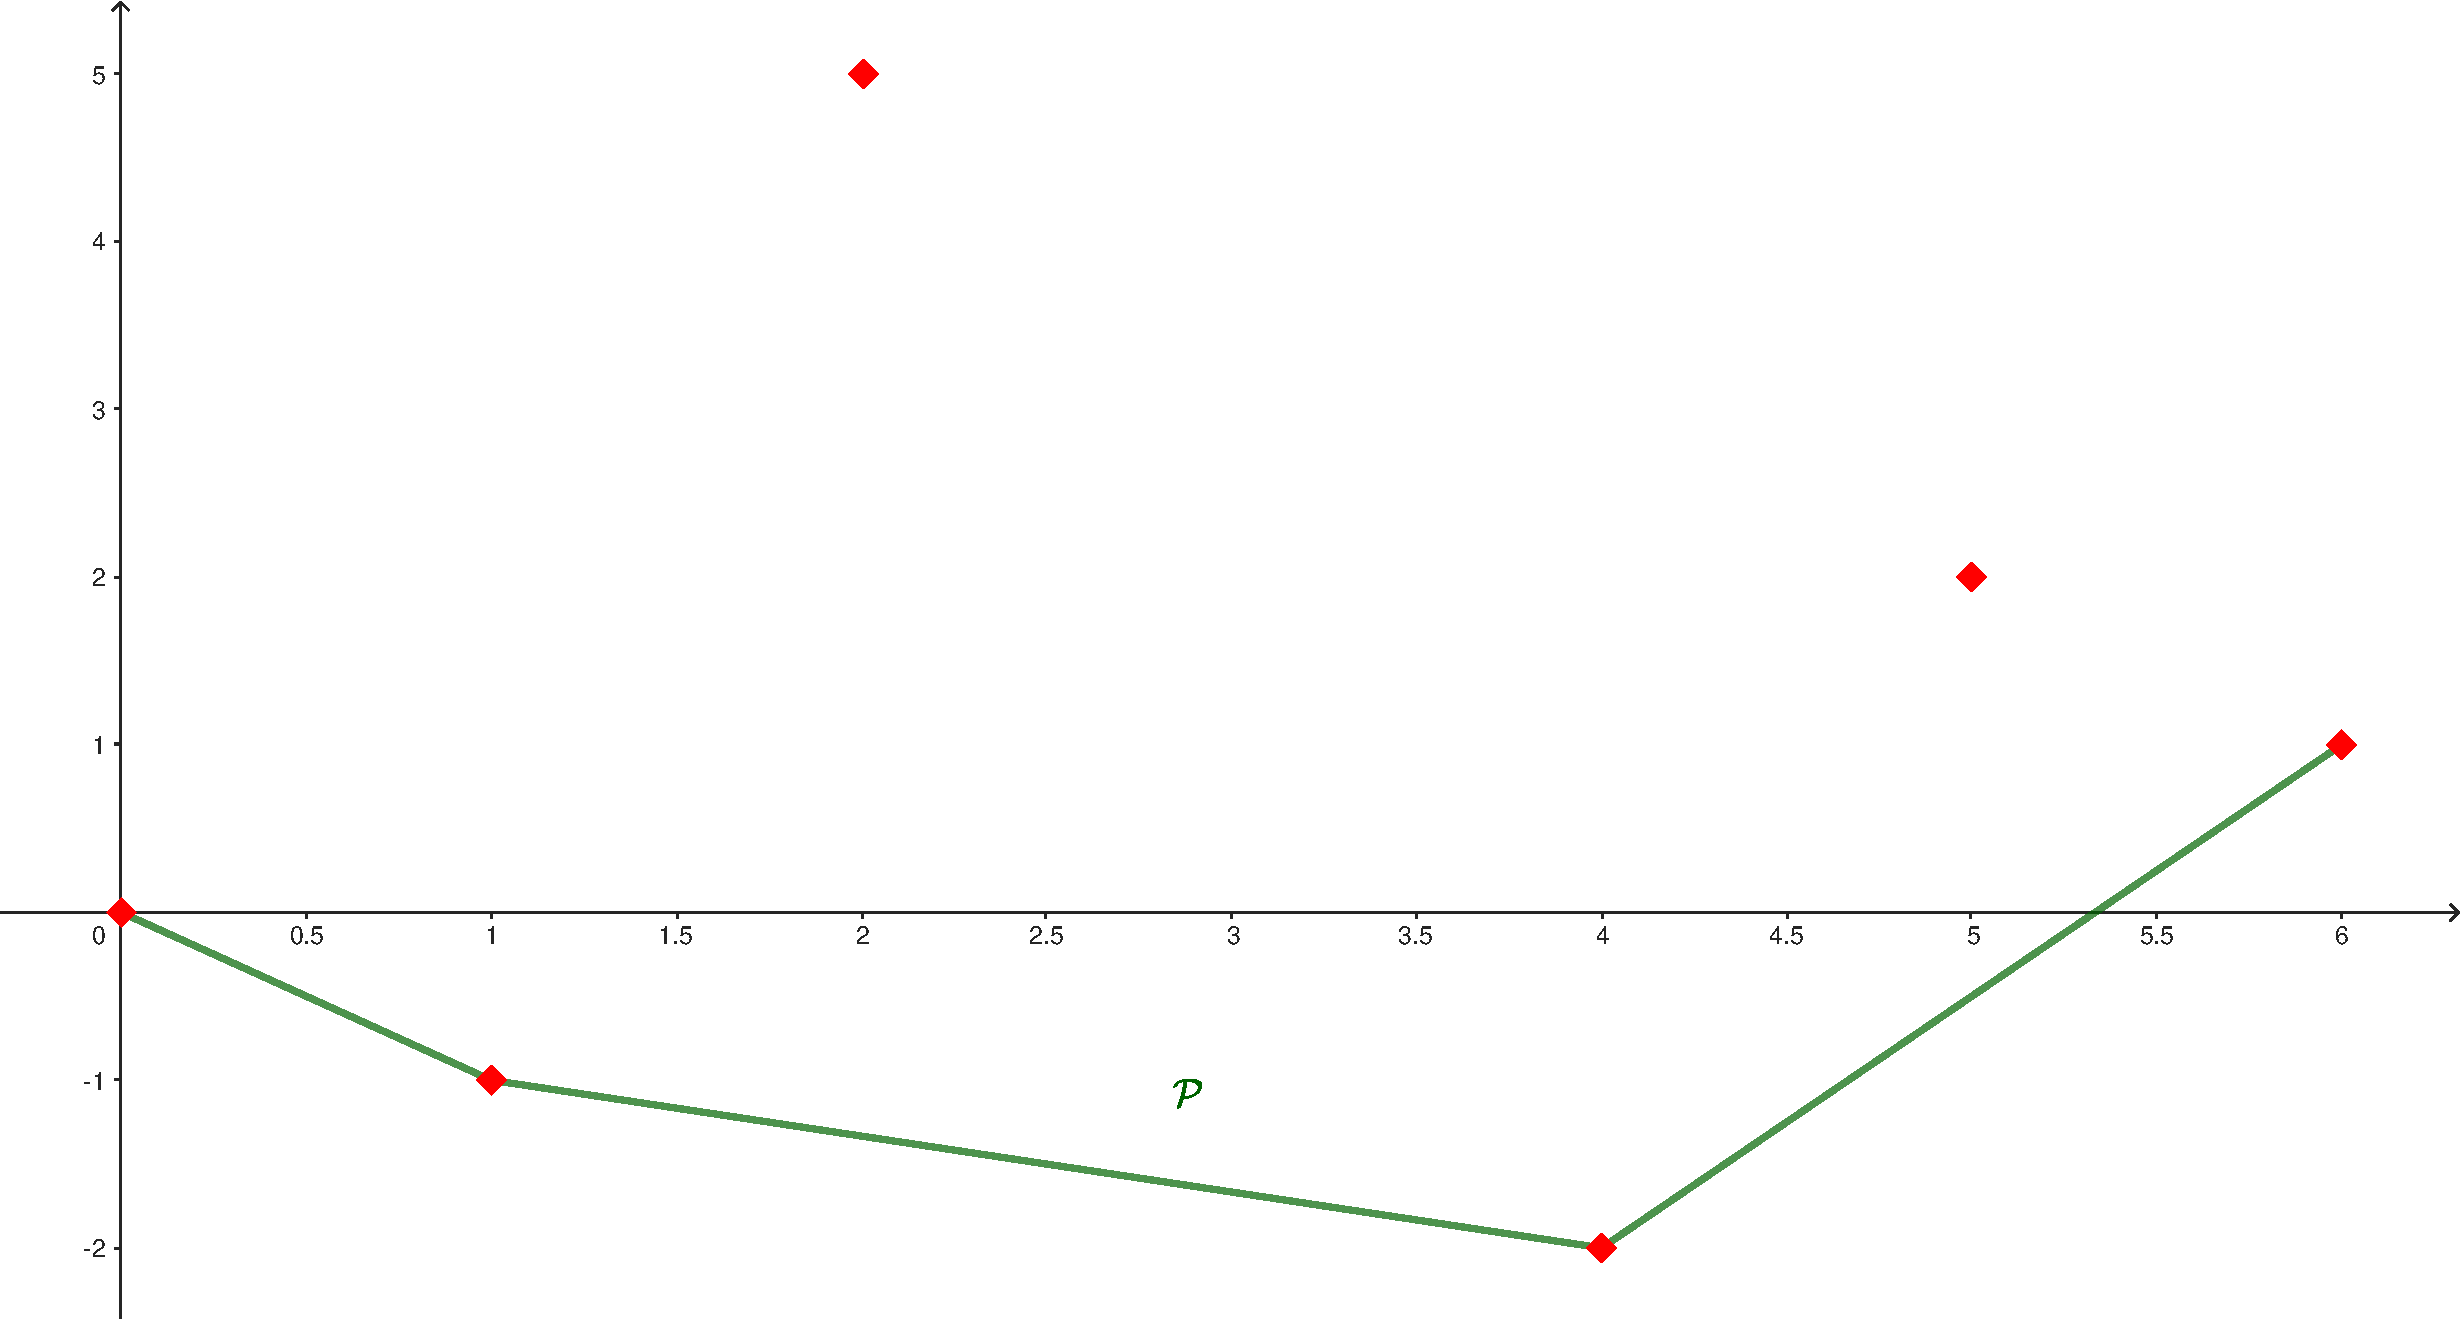
\includegraphics[scale=0.25]{figures/polygone_newton.pdf}
      \caption{Polygone de Newton $\mathcal{P}$ associé à $P$}
      \label{poly_newton}
    \end{figure}
  \end{ex}

On pourra alors prouver que l'enveloppe convexe inférieure ainsi définie est une ligne brisée constitués de segments de pentes deux à deux différentes. On appelle pentes du polygones les pentes des segments de la ligne brisée et longueur d'un segment de la ligne brisé la longueur du projeté du segment sur l'axe des abscisses. 

\begin{theoreme}
Les pentes du polygone de Newton $\mathcal{P}$ sont exactement les opposés des valuations des racines de $P$ (dans $\overline{\mathbb{Q}_{p}}$). De plus, le nombre de racines de valuation $v$ est égal à la longueur du segment de pente $-v$.
\end{theoreme}

On considère alors un polynôme $P =X^n \sum_{i=1}^{n-1} a_{i}X^i$ à coefficient dans $\mathbb{Q}_p$ unitaire. On remarque immédiatement que le point d'abscisse $n$ du polygone de Newton $\mathcal{P}$ associé à $P$ est d'ordonnée nulle. On en déduit alors que si un des coefficients $(a_{i})_{0\le i\le n-1}$ est de valuation strictement négative, $\mathcal{P}$ admet une pente strictement positive et donc $P$ admet une racine de valuation strictement négative. 

Par contraposée, on en déduit que si polynôme unitaire à coefficient dans $\mathbb{Q}_{p} $ est à racine positive alors il est élément de $\mathbb{Z}_p[X]$.
>>>>>>> afed46df6ee66c8447d25c77be41fc228335ae00

\end{proof} 
